% This file was created by matplotlib2tikz v0.7.5.
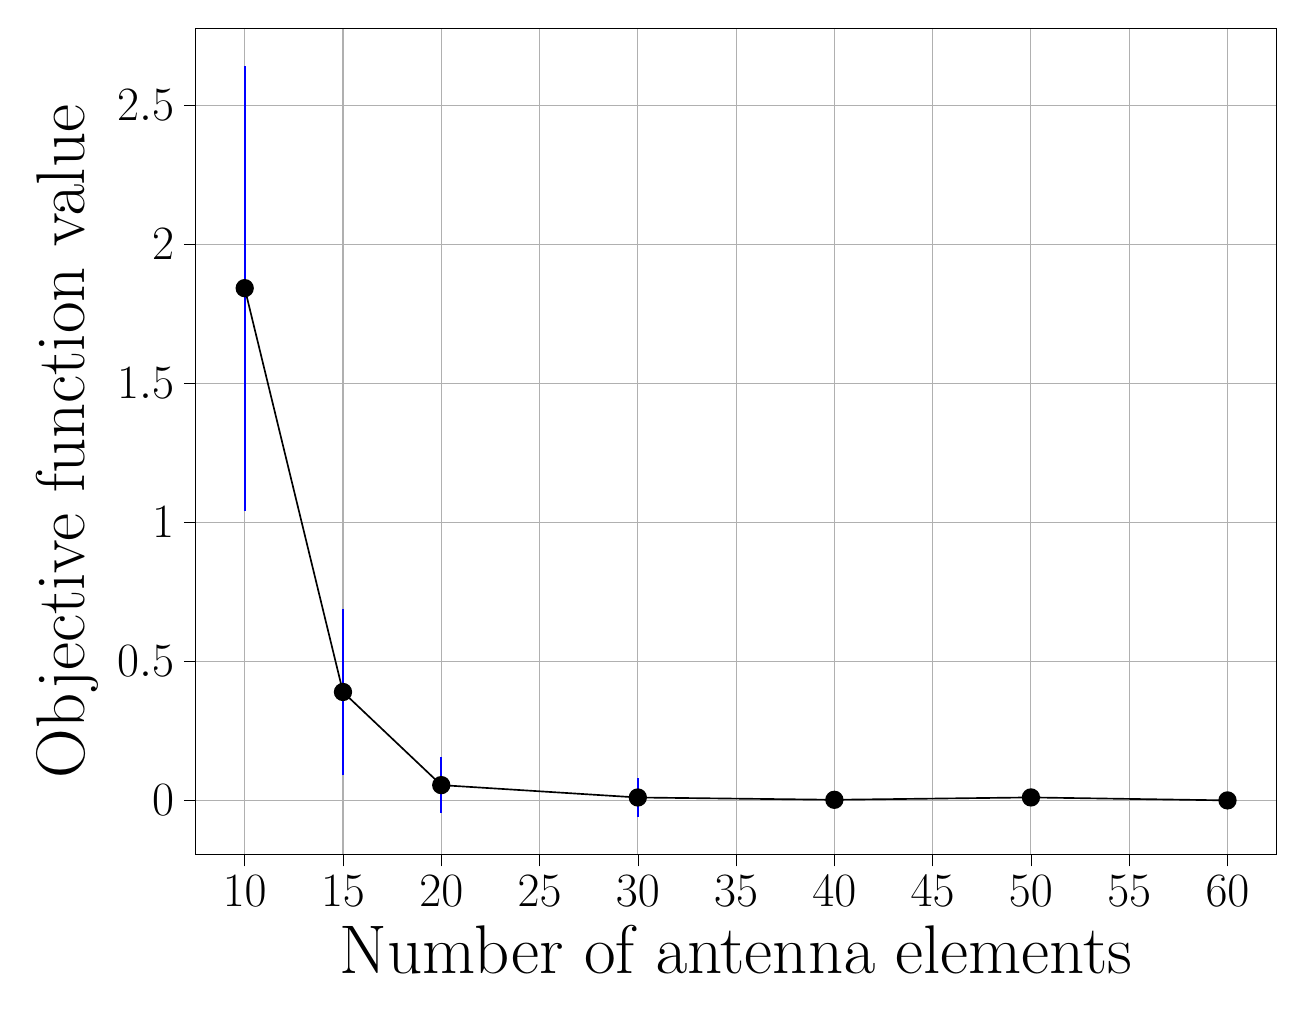
\begin{tikzpicture}

\begin{axis}[
width=6.028in,
height=4.754in,
xlabel style={font=\Huge},
ticklabel style={font=\LARGE},
ylabel style={font=\Huge},
tick align=outside,
tick pos=left,
x grid style={white!69.01960784313725!black},
xlabel={Number of antenna elements},
xmajorgrids,
xmin=7.5, xmax=62.5,
xtick style={color=black},
y grid style={white!69.01960784313725!black},
ylabel={Objective function value},
ymajorgrids,
ymin=-0.194615, ymax=2.777915,
ytick style={color=black}
]
\path [draw=blue, thick]
(axis cs:10,1.0428)
--(axis cs:10,2.6428);

\path [draw=blue, thick]
(axis cs:15,0.09)
--(axis cs:15,0.69);

\path [draw=blue, thick]
(axis cs:20,-0.045)
--(axis cs:20,0.155);

\path [draw=blue, thick]
(axis cs:30,-0.0595)
--(axis cs:30,0.0805);

\path [draw=blue, thick]
(axis cs:40,-0.0078)
--(axis cs:40,0.0122);

\path [draw=blue, thick]
(axis cs:50,0.0107)
--(axis cs:50,0.0107);

\path [draw=blue, thick]
(axis cs:60,0)
--(axis cs:60,0);

\addplot [semithick, black, mark=*, mark size=3, mark options={solid}]
table {%
10 1.8428
15 0.39
20 0.055
30 0.0105
40 0.0022
50 0.0107
60 0
};
\end{axis}

\end{tikzpicture}